\chapter{CUDA Synchronisations}

\newcommand{\code}[1]{\texttt{#1}}
\newcommand{\synct}{\code{\_\_syncthreads()}}

\section{Introduction to GPUs and CUDA}

Graphics Processing Units (GPUs) have emerged as a powerful platform for high-performance parallel computing. Originally designed for rendering graphics, modern GPUs are now widely used for general-purpose computation in domains such as scientific computing, machine learning, and large-scale data processing.

\subsection{GPU vs CPU: Design Philosophy}

The fundamental difference between CPUs and GPUs lies in their design goals. CPUs are optimized for executing a small number of threads with very low latency. This is achieved through sophisticated control logic, deep cache hierarchies, branch prediction, and out-of-order execution. In contrast, GPUs are designed to execute thousands of threads concurrently with high throughput. \cite{gpu_lecture}

GPUs achieve this by:
\begin{itemize}
    \item Using a large number of simpler cores operating at lower clock speeds
    \item Employing a Single Instruction Multiple Threads (SIMT) execution model
    \item Reducing control complexity and cache size
    \item Providing extremely high memory bandwidth (up to terabytes per second)
\end{itemize}

This architectural difference makes GPUs highly efficient for data-parallel workloads where the same operation is applied to many data elements simultaneously.

\subsection{GPU Architecture Overview}

A modern GPU consists of multiple Streaming Multiprocessors (SMs), each containing several processing cores, registers, shared memory, and specialized units such as tensor cores. The GPU is connected to the host CPU via high-speed interconnects such as PCI-Express. 

Each SM executes groups of threads called \textit{warps}, typically consisting of 32 threads that execute instructions in lock-step. This execution model enables efficient utilization of hardware resources but also introduces challenges such as warp divergence when threads follow different execution paths.

The memory hierarchy in GPUs includes:
\begin{itemize}
    \item Registers (per-thread, fastest)
    \item Shared memory (per-block, low latency)
    \item L1 and L2 caches
    \item Global memory (high latency, large capacity)
\end{itemize}

Efficient GPU programming requires careful management of this memory hierarchy to maximize performance. 

\subsection{GPU Model of Computation}

GPU computation follows a heterogeneous programming model where execution is divided between the host (CPU) and the device (GPU). The host is responsible for orchestrating the computation, including memory allocation, data transfer, and kernel launches, while the device performs the actual parallel computation. \cite{cuda_lecture}

The computation on the GPU is expressed in terms of \textit{kernels}, which are functions executed by many threads in parallel. Threads are organized hierarchically:
\begin{itemize}
    \item Threads form thread blocks
    \item Thread blocks form a grid
\end{itemize}

Each thread performs a portion of the computation, enabling massive parallelism. Thread blocks are scheduled on Streaming Multiprocessors, and threads within a block can cooperate using shared memory. \cite{cuda_lecture}

\subsection{Introduction to CUDA}

CUDA (Compute Unified Device Architecture) is a parallel programming framework developed by NVIDIA that allows programmers to write code for GPUs using extensions to C/C++. CUDA provides an abstraction for managing the GPU execution model and memory hierarchy.

In CUDA, programs consist of:
\begin{itemize}
    \item Host code: Runs on the CPU and manages execution
    \item Device code: Runs on the GPU as kernels
\end{itemize}

Kernel execution is initiated by the host and executed asynchronously on the device. Multiple kernels can be launched concurrently using streams, enabling overlap of computation and data transfer. \cite{cuda_lecture}

\subsection{Execution Workflow}

A typical CUDA program follows these steps:
\begin{enumerate}
    \item Allocate memory on the device
    \item Transfer data from host to device
    \item Launch kernel with specified grid and block dimensions
    \item Execute computation in parallel on the GPU
    \item Transfer results back to the host
\end{enumerate}

This workflow highlights the importance of data movement and parallel execution in GPU computing.

\subsection{Summary}

GPUs provide a massively parallel architecture optimized for throughput-oriented workloads. CUDA enables developers to harness this computational power through a structured programming model that separates host and device responsibilities. Understanding the architectural principles and execution model of GPUs is essential for writing efficient parallel programs.
\newpage
\section{CUDA Basics}

CUDA (Compute Unified Device Architecture) provides a programming model that enables developers to utilize the massive parallelism offered by GPUs. In this section, we introduce the fundamental concepts required to understand CUDA programming.

\subsection{Kernels}

A \textit{kernel} is the basic unit of execution on the GPU. It is a function that is executed in parallel by a large number of threads on the device. Kernels are defined using the \texttt{\_\_global\_\_} qualifier, indicating that they run on the GPU but are invoked from the host (CPU). \cite{cuda_lecture}

\begin{lstlisting}[language=C++]
__global__ void vector_add(const float *A, const float *B, float *C, int N)
{
    int i = blockIdx.x * blockDim.x + threadIdx.x;

    if (i < N)
        C[i] = A[i] + B[i];
}
\end{lstlisting}

The conditional check \texttt{if (i < N)} is necessary because the total number of threads launched is often rounded up to cover all data elements. As a result, some threads may compute indices beyond the valid range of the input arrays. This check prevents out-of-bounds memory access, ensuring correctness and avoiding undefined behavior.

\subsection{Thread Hierarchy}

CUDA organizes threads in a hierarchical structure to enable scalable parallelism:

\begin{itemize}
    \item \textbf{Thread:} Smallest unit of execution. Each thread performs a portion of the computation.
    \item \textbf{Block:} A group of threads that can cooperate via shared memory and synchronize with each other.
    \item \textbf{Grid:} A collection of thread blocks executing the same kernel.
\end{itemize}

\subsection{Thread Indexing}

In CUDA, each thread is uniquely identified using built-in variables such as \texttt{threadIdx}, \texttt{blockIdx}, and \texttt{blockDim}. These variables allow mapping each thread to a specific portion of the data.

Within a block, threads are indexed using \texttt{threadIdx.x}, which ranges from $0$ to $\texttt{blockDim.x} - 1$. Similarly, each block in a grid is identified by \texttt{blockIdx.x}.

To compute a unique global index for each thread across all blocks, the following formula is used:

\begin{equation}
\text{index} = \texttt{threadIdx.x} + \texttt{blockIdx.x} \times \texttt{blockDim.x}
\end{equation}

This formula ensures that:
\begin{itemize}
    \item Threads within a block access consecutive indices
    \item Different blocks process different portions of the data
\end{itemize}

For example, if each block contains 8 threads and there are multiple blocks, then:
\begin{itemize}
    \item Block 0 handles indices $0$ to $7$
    \item Block 1 handles indices $8$ to $15$
    \item Block 2 handles indices $16$ to $23$, and so on
\end{itemize}

This indexing scheme enables scalable parallelization, allowing CUDA programs to efficiently distribute work across thousands of threads.


\subsection{Execution Model}

CUDA follows a heterogeneous execution model where:

\begin{itemize}
    \item The \textbf{host (CPU)} manages memory allocation, data transfers, and kernel launches.
    \item The \textbf{device (GPU)} executes kernels in parallel.
\end{itemize}

Kernel launches are asynchronous by default, meaning the CPU does not wait for GPU execution to complete unless explicitly synchronized.

\subsection{Kernel Invocation}

Kernels are launched from the host using the following syntax:

\begin{lstlisting}[language=C++]
int threads_per_block = 256;
int blocks = (N + threads_per_block - 1) / threads_per_block;

vector_add<<<blocks, threads_per_block>>>(d_A, d_B, d_C, N);
cudaDeviceSynchronize();
\end{lstlisting}

Here:
\begin{itemize}
    \item \texttt{threads\_per\_block} defines the number of threads in each block.
    \item \texttt{blocks} defines the number of blocks in the grid.
    \item \texttt{cudaDeviceSynchronize()} ensures that the host waits for GPU execution to complete.
\end{itemize}

\subsection{Memory Management}

CUDA provides explicit control over memory allocation and data transfer between host and device.

\begin{lstlisting}[language=C++]
// Device memory allocation
cudaMalloc(&d_A, bytes);
cudaMalloc(&d_B, bytes);
cudaMalloc(&d_C, bytes);

// Copy data from host to device
cudaMemcpy(d_A, h_A, bytes, cudaMemcpyHostToDevice);
cudaMemcpy(d_B, h_B, bytes, cudaMemcpyHostToDevice);

// Copy results back to host
cudaMemcpy(h_C, d_C, bytes, cudaMemcpyDeviceToHost);
\end{lstlisting}

Data transfers between host and device are relatively expensive and should be minimized for better performance.

\subsection{Device Qualifiers}

CUDA uses special qualifiers to specify where functions execute and where they are called from:

\begin{itemize}
    \item \texttt{\_\_global\_\_}: Executed on the device, called from the host (used for kernels)
    \item \texttt{\_\_device\_\_}: Executed and called on the device (helper functions)
    \item \texttt{\_\_host\_\_}: Executed on the host (default C/C++ functions)
\end{itemize}

\subsection{Memory Types}

CUDA provides different memory spaces with varying scope and performance characteristics:

\begin{itemize}
    \item \textbf{Registers:} Fastest, private to each thread
    \item \textbf{Shared Memory:} Fast, shared among threads in a block
    \item \textbf{Global Memory:} Large but high latency, accessible by all threads
    \item \textbf{Constant Memory:} Read-only, cached memory for constant data
\end{itemize}

Efficient utilization of these memory types is crucial for achieving high performance.

\subsection{Summary}

CUDA abstracts the complexity of GPU programming through kernels, thread hierarchies, and explicit memory management. By organizing computation into grids, blocks, and threads, and carefully managing memory and synchronization, developers can exploit the massive parallelism offered by modern GPUs.

\subsection{Exercises}
\begin{ppexercises}

\ppexercise{%
\textbf{GPU Architecture and SIMT:}
Consider a GPU where each Streaming Multiprocessor (SM) handles warps of 32 threads.

\begin{enumerate}[label=(\alph*)]
\item Explain the concept of \textit{warp divergence}. What happens to the execution throughput when an \texttt{if-else} statement causes half the threads in a warp to take one path and the other half to take another?
\item Why does the GPU architecture prefer many simple cores over a few complex cores like a CPU?
\item If a kernel is launched with a block size of 40 threads, how many warps are scheduled for that block? Justify your answer.
\end{enumerate}
}

\ppexercise{%
\textbf{Thread Indexing and Mapping:}
A programmer wants to process a 1D array of size N=1000. They decide to use a block size (\texttt{blockDim.x}) of 256 threads.

\begin{enumerate}[label=(\alph*)]
\item Calculate the minimum number of blocks required to cover all elements.
\item Provide the specific CUDA kernel launch syntax (the \texttt{<<<...>>>} part) for this configuration.
\item Inside the kernel, a thread belongs to \texttt{blockIdx.x = 2} and has \texttt{threadIdx.x = 10}. What is the global index i this thread will calculate?
\item Explain why the condition \texttt{if (i < N)} is strictly necessary in this specific scenario.
\end{enumerate}
}

\ppexercise{%
\textbf{Memory Hierarchy and Latency:}
CUDA programmers must choose between Global, Shared, and Register memory.

\begin{enumerate}[label=(\alph*)]
\item Arrange the three memory types (Global, Shared, Registers) in order of increasing capacity and increasing latency.
\item In a vector addition kernel (C=A+B), the variables A,B, and C are stored in Global Memory. If the kernel is limited by the time it takes to fetch these values, is it "compute-bound" or "memory-bound"?
\item Why is \texttt{cudaMemcpy} considered a potential bottleneck in a heterogeneous computing workflow?
\end{enumerate}
}

\end{ppexercises}

\subsection*{Solutions}

\subsubsection{Solution 1}

\begin{enumerate}[label=(\alph*)]
\item \textbf{Warp Divergence:} Since threads in a warp execute in lock-step (SIMT), if they diverge, the hardware must serialize the paths. It executes the \texttt{if} path while masking the \texttt{else} threads, then vice versa. This can drop throughput by up to 50% in this specific case.
\item \textbf{Throughput vs. Latency:} CPUs use complex logic to minimize the latency of a single thread. GPUs sacrifice per-thread latency and complex logic to maximize total throughput, using the area to pack more arithmetic units (ALUs).
\item \textbf{Warp Scheduling:} 2 warps. Warps are always allocated in groups of 32 threads. 40/32=1.25, which rounds up to 2 warps (64 slots total, with 24 threads being inactive).
\end{enumerate}

\subsubsection{Solution 2}
% \begin{enumerate}[label=(\alph*)]
% \item \textbf{Number of Blocks.} To find the number of blocks B required for an array of size N with a block size T, we use the ceiling division:


% \item \textbf{Kernel Launch Syntax.} Using the calculated dimensions (4 blocks, 256 threads):
% \begin{lstlisting}[language=C++]
% // Launching the kernel with 4 blocks of 256 threads each
% vector_add<<<4, 256>>>(d_A, d_B, d_C, N);
% \end{lstlisting}

% \item \textbf{Global Index Calculation.} The unique global index i is calculated using the formula:
% \begin{align*}
% i &= \text{threadIdx.x} + (\text{blockIdx.x} \times \text{blockDim.x}) \
% \end{align*}
% \begin{align*}
% i &= 10 + (2 \times 256) \ = 10 + 512 = \mathbf{522}.
% \end{align*}
    

% \item \textbf{Necessity of Boundary Guards.}
% With 4 blocks of 256 threads, the GPU launches a total of 4×256=1024 threads. Since the array size N is only 1000, threads with global indices i belongs to [1000,1023] would attempt to access memory beyond the allocated bounds of the arrays. The \texttt{if (i < N)} guard ensures these "extra" threads remain idle, preventing memory corruption or undefined behavior.
% \end{enumerate}

\begin{enumerate}[label=(\alph*)]
  \item \textbf{Number of Blocks.} To find the number of blocks B required for an array of size N with a block size T, we use the ceiling division: B = 1000/256 == 4.

\item \textbf{Kernel Launch Syntax.} Using the calculated dimensions (4 blocks, 256 threads):
\begin{lstlisting}[language=C++]
// Launching the kernel with 4 blocks of 256 threads each
vector_add<<<4, 256>>>(d_A, d_B, d_C, N);
\end{lstlisting}

\item \textbf{Global Index Calculation.} The unique global index i is calculated using the formula:
        \begin{align*}
          i &= \text{threadIdx.x} + (\text{blockIdx.x} \times \text{blockDim.x}) \
        \end{align*}
        \begin{align*}
            i &= 10 + (2 \times 256) = 10 + 512 = \mathbf{522}
        \end{align*}

\item \textbf{Necessity of Boundary Guards.}
With 4 blocks of 256 threads, the GPU launches a total of 4×256=1024 threads. Since the array size N is only 1000, threads with global indices i belongs in [1000,1023] would attempt to access memory beyond the allocated bounds of the arrays. The \texttt{if (i < N)} guard ensures these "extra" threads remain idle, preventing memory corruption or undefined behavior.
\end{enumerate}

\subsubsection{Solution 3}
\begin{enumerate}[label=(\alph*)]
\item \textbf{Hierarchy:}
\begin{itemize}
\item \textbf{Capacity:} Registers < Shared Memory < Global Memory
\item \textbf{Latency:} Registers < Shared Memory < Global Memory
\end{itemize}
\item \textbf{Bottleneck:} It is \textbf{memory-bound}. The performance is limited by the high latency and bandwidth limits of Global Memory rather than the speed of the floating-point units.
\item \textbf{PCIe Overhead:} Data must travel over the PCIe bus, which has much lower bandwidth than the GPU's internal memory. Moving data often takes longer than the actual calculation.
\end{enumerate}
\newpage
% ─────────────────────────────────────────────────────────────────────────────
\section{Revisiting the Memory Hierarchy}
\label{sec:memory-hierarchy}
% ─────────────────────────────────────────────────────────────────────────────

Before delving into the intricacies of shared-memory programming, it is imperative to briefly revisit the memory hierarchy of a modern GPU. Understanding the distinct memory spaces, their physical locations, and their accessibility scopes is crucial for writing performant CUDA kernels.

The GPU memory architecture comprises several distinct layers, ranging from small, exceptionally fast on-chip memory to large, high-latency off-chip memory:
l
\begin{itemize}
    \item \textbf{Registers:} These are strictly on-chip and are private to each individual thread. They offer the lowest latency and highest bandwidth of all memory spaces.
    
    \item \textbf{Shared memory:} This is a fast, on-chip memory space that is shared by all threads residing within the \textbf{same block}. Because it is explicitly managed by the programmer, it serves as a highly efficient block-level scratch-pad.
    
    \item \textbf{L1 Cache/ Read-only Cache/ Texture Cache:} These are on-chip memory structures managed entirely by the hardware. They help buffer global memory accesses and exploit spatial and temporal locality without explicit programmer intervention.
    
    \item \textbf{L2 Cache:} This is a large on-chip cache that serves as a unified backing store, shared across all Streaming Multiprocessors (SMs).
    
    \item \textbf{Global Memory:} This is the largest memory space available on the device, but it is also markedly slow. Data that must be persistent across kernel launches or is too large to fit in on-chip memory resides here.
\end{itemize}
\newpage
\section{Shared-Memory Usage}


\subsection{Overview}
 
Having introduced the memory hierarchy of GPUs and the role of shared memory
as a fast, programmer-managed scratchpad, the instructor turned to a concrete
worked example: the \textbf{stencil based computation}. This example is a
canonical shared-memory use case because it exhibits significant data reuse,
each input element is accessed by multiple neighbouring threads, making it
an ideal vehicle for demonstrating how a naive global-memory kernel can be
transformed into an efficient shared-memory kernel.
 
% ── Slide 1 ──────────────────────────────────────────────────────────────────
\subsection{Stencil Computation: The Naive Global-Memory Kernel}

 
\subsubsection{What Is a Stencil Computation?}
 
A \textbf{stencil computation} is a grid-based computation in which the output
at each grid point depends on the values of its neighbours. In the 1-D case,
the output at index~$i$ depends on the elements at indices $i-1$, $i$, and
$i+1$:
 
\[
  B[i] \;=\; A[i-1] + A[i] + A[i+1], \qquad 0 < i < N-1.
\]
 
Stencil computations are very common in scientific computing, examples
include finite-difference solvers for partial differential equations and image
processing filters. They also appear naturally in the matrix-transpose problem,
another classic shared-memory exercise.
 
\subsubsection{Naive Kernel: Direct Global-Memory Reads}
 
The simplest possible CUDA implementation assigns one thread to each output
element and reads the three needed input values directly from global memory:
 

\begin{ppprogram}{Naive Implementation (Slide 8)}{lst:label}
\begin{lstlisting}[language=C++]
__global__ void stencil_naive(const float *A, float *B, int N) {
    int i = blockIdx.x * blockDim.x + threadIdx.x;
    
    if (i > 0 && i < N - 1) {
        B[i] = A[i - 1] + A[i] + A[i + 1];
    }
}
\end{lstlisting}
\end{ppprogram}
 
The guard \texttt{i > 0 \&\& i < N - 1} prevents out-of-bounds accesses at
the two endpoints of the array.
 
\subsubsection{Why Is This Naive?}
 
Even though the computation is straightforward, the access pattern is highly
inefficient. For each output element, three separate global-memory reads are
issued. Crucially, the element \texttt{A[i]} that thread~$i$ reads as its
``centre'' value is \emph{also} read by thread~$i-1$ (as its right neighbour)
and by thread~$i+1$ (as its left neighbour). Every element is therefore read
\textbf{three times from global memory}. With a global-memory latency of
roughly 800 cycles, this redundancy is extremely costly.
 
\begin{ppkey}
  \\The insight motivating shared memory here is \textbf{locality and reuse}.
  Although the L1 cache would capture some of this reuse automatically, it
  cannot be \emph{relied upon}: the hardware's cache-replacement policy may
  evict a line before all threads that need it have executed. Shared memory,
  by contrast, is under explicit programmer control, so the data is guaranteed
  to remain available for the entire duration of the block's computation.
  Shared memory access latency is approximately 5--7 cycles versus
  $\sim$800 cycles for global memory which is a two-order-of-magnitude improvement.
\end{ppkey}
 
\begin{ppnote}
  \\\textbf{Student question:} Won't the L1 cache handle this automatically?\\[4pt]
  \textbf{Instructor:} Yes, the L1 cache will be used, and for \emph{this}
  specific example it would help. But the L1 cache is hardware-controlled with
  primitive replacement logic, it cannot guarantee that overlapping accesses
  from different threads remain resident. With shared memory you have explicit
  control at programming time. The L1 cache is a useful backstop; shared
  memory is a deliberate optimisation strategy. There are workloads where the
  L1 cache simply would not suffice, and shared memory is the correct tool.
\end{ppnote}
 
\subsubsection{The Fix: Load a Window into Shared Memory}
 
The solution is to \textbf{load a window of global memory into shared memory}
before performing the stencil computation. Each thread block cooperatively
loads the global-memory elements it needs into a shared array
\texttt{sA[]}. Subsequent reads then hit shared memory instead of global
memory.
 
The window loaded must include not only the elements owned by the block's
threads, but also the \textbf{halo} (or \textbf{ghost cell}) elements: the
one element immediately to the left of the block's leftmost thread, and the
one element immediately to the right of its rightmost thread. These boundary
elements are required by the leftmost and rightmost threads of the block to
complete their stencil computations, but they are \emph{owned} by adjacent
blocks.

\begin{figure}[!h]
    \centering
    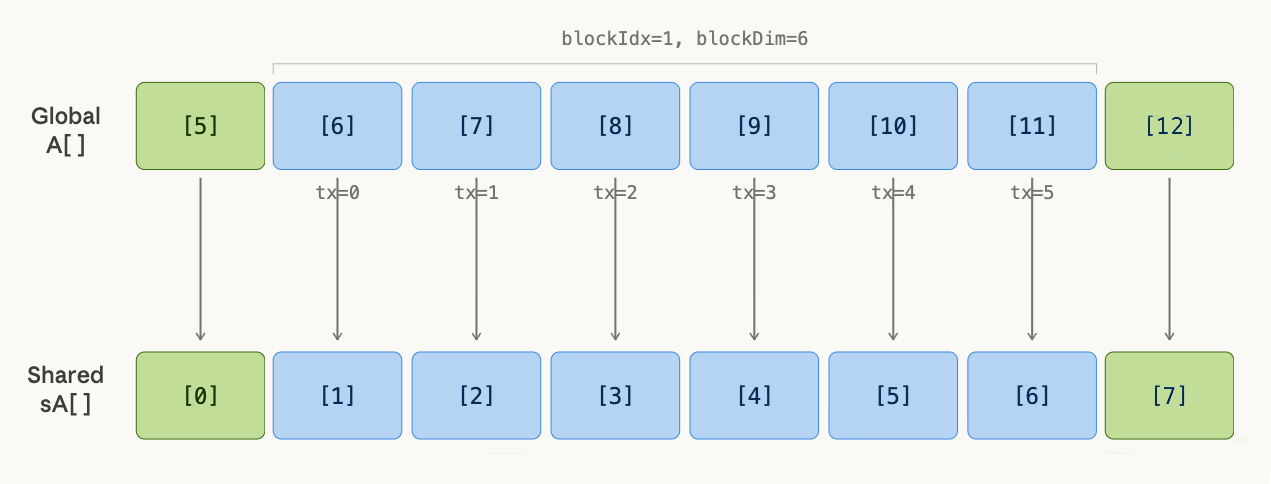
\includegraphics[width=1\linewidth]{images/withhalo.png}
    \caption{
    Mapping of global memory array \texttt{A[]} to shared memory array \texttt{sA[]} 
    in the \texttt{stencil\_shared} kernel for \texttt{blockDim.x = 6} and 
    \texttt{blockIdx.x = 1}.
    }
    \label{fig:shared-mapping}
    
\end{figure}
 
% ── Slide 2 ──────────────────────────────────────────────────────────────────
\subsection{Loading Center Elements into Shared Memory}

 
\subsubsection{Shared-Memory Array Layout}
 
For a block of dimension \texttt{blockDim.x}, the shared array is declared
with \textbf{two extra slots}, one on each side to accommodate the left and
right halo elements:

\begin{ppprogram}{Loading Center Elements (Slide 9)}{lst:label}
\begin{lstlisting}[language=C++]
__global__ void stencil_shared(const float *A, float *B, int N) {
    __shared__ float sA[256 + 2];  // blockDim.x assumed 256;
                                   // +2 for left and right halos
 
    int tx = threadIdx.x;
    int i  = blockIdx.x * blockDim.x + tx;
 
    // Load center element: A[i] goes into sA[tx + 1]
    // (index 0 is reserved for the left halo)
    if (i < N) {
        sA[tx + 1] = A[i];
    }
    ...
\end{lstlisting}
\end{ppprogram}

This particular part of code is responsible for loading the center elements into the shared memory which are depicted by blue in Figure \ref{fig:shared-mapping}.
 
The offset \texttt{tx + 1} is deliberate: index~0 of \texttt{sA[]} is
reserved for the left halo element, so the thread-owned center elements occupy
positions 1 through \texttt{blockDim.x}. The right halo will occupy position
\texttt{blockDim.x + 1}.
 
\subsubsection{Worked Example: \texttt{blockDim.x = 6}, \texttt{blockIdx.x = 1}}
 
To make the indexing concrete, the instructor worked through the case
\texttt{blockDim.x = 6} (chosen for clarity) and \texttt{blockIdx.x = 1}.
The global indices for this block are:
 
\[
  i \;=\; 1 \times 6 + tx \;\in\; [6,\,11], \quad tx \in [0,5].
\]
 
The center-element load maps as follows:
 \begin{figure}[!h]
    \centering
    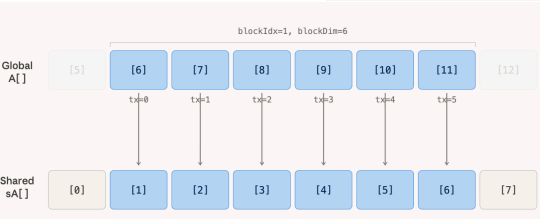
\includegraphics[width=0.8\linewidth]{images/shared.png}
    \label{fig:no-halo}
    
\end{figure}
 
The slots \texttt{sA[0]} and \texttt{sA[7]} are left empty at this stage;
they will be filled when the halo elements are loaded.

% ── Slide 3 ──────────────────────────────────────────────────────────────────
\subsection{Loading Halo Elements and Synchronising}

 
\subsubsection{Why Halo Elements Are Needed}
 
At the block boundary, the leftmost thread (\texttt{tx = 0}) of a block
requires the element \texttt{A[i-1]}, which belongs to the \emph{last} thread
of the preceding block. Similarly, the rightmost thread
(\texttt{tx = blockDim.x - 1}) requires \texttt{A[i+1]}, owned by the
\emph{first} thread of the following block. These boundary elements are called
\textbf{halo regions} or \textbf{ghost cells}. They must be explicitly loaded
into the shared array before the stencil computation can proceed.
 
\subsubsection{Loading the Left Halo}
 
Only the \emph{first thread} of a block (\texttt{tx == 0}) is responsible for
loading the left halo. An additional guard \texttt{i > 0} prevents an
out-of-bounds read when the block is the very first block in the grid (i.e.\
\texttt{blockIdx.x == 0}), for which no left neighbour exists:
 
\begin{ppprogram}{Load Left Halo (Slide 10)}{lst:label}
\begin{lstlisting}[language=C++]
// Load left halo
if (tx == 0 && i > 0) {
    sA[0] = A[i - 1];
}
\end{lstlisting}
\end{ppprogram}

The left halo loads as follows:
 \begin{figure}[!h]
    \centering
    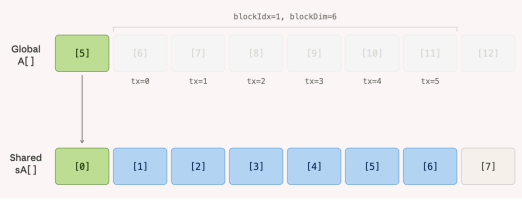
\includegraphics[width=0.8\linewidth]{images/sharedhalo.png}
    \label{fig:one-halo}
    
\end{figure}
 
\subsubsection{Loading the Right Halo}
 
Symmetrically, only the \emph{last thread} of a block loads the right halo,
guarded by \texttt{i < N - 1} to avoid reading past the end of the array:
 
\begin{ppprogram}{Load Right Halo (Slide 10)}{lst:label}
\begin{lstlisting}[language=C++]
// Load right halo
if (tx == blockDim.x - 1 && i < N - 1) {
    sA[blockDim.x + 1] = A[i + 1];
}
\end{lstlisting}
\end{ppprogram}

After every thread has executed its center and halo loads, the shared array is fully populated and looks like Figure \ref{fig:shared-mapping}.
 
\subsubsection{The Synchronisation Barrier: \texttt{\_\_syncthreads()}}
 
After all center and halo elements have been written into \texttt{sA[]}, the
shared array is fully populated. However, the writes are performed by
different threads, which may execute at different speeds. Without an explicit
synchronisation point, a thread could advance to the stencil computation phase
and read a shared-memory slot that has not yet been written by the responsible
thread, this rises a \textbf{race condition}.
 
The solution is \texttt{\_\_syncthreads()}, placed immediately after all
shared-memory stores:


\begin{ppprogram}{Sync Barrier (Slide 10)}{lst:label}
\begin{lstlisting}[language=C++]
__global__ void stencil_shared(const float *A, float *B, int N) {
    __shared__ float sA[256 + 2];   // blockDim.x assumed 256
 
    int tx = threadIdx.x;
    int i  = blockIdx.x * blockDim.x + tx;
 
    // Phase 1: populate shared memory 
    // Center element
    if (i < N)
        sA[tx + 1] = A[i];
 
    // Left halo (only thread 0 of each non-first block)
    if (tx == 0 && i > 0)
        sA[0] = A[i - 1];
 
    // Right halo (only last thread of each non-last block)
    if (tx == blockDim.x - 1 && i < N - 1)
        sA[blockDim.x + 1] = A[i + 1];
 
    // Barrier: all shared-memory stores must complete 
    __syncthreads();
 
    // Phase 2: stencil computation using shared memory
    if (i > 0 && i < N - 1)
        B[i] = sA[tx] + sA[tx + 1] + sA[tx + 2];
}
\end{lstlisting}
\end{ppprogram}
 
Notice how the final computation replaces every global-memory read with a
shared-memory read: \texttt{A[i-1]}, \texttt{A[i]}, \texttt{A[i+1]} become
\texttt{sA[tx]}, \texttt{sA[tx+1]}, \texttt{sA[tx+2]}. This is the payoff
for the setup work done in Phase~1.
 
\subsubsection{Dual Role of \texttt{\_\_syncthreads()}}
 
\texttt{\_\_syncthreads()} simultaneously provides two guarantees (from slide
10):
 
\begin{enumerate}
  \item \textbf{Execution barrier.} No thread in the block may execute any
        instruction beyond the \texttt{\_\_syncthreads()} call until
        \emph{every} thread in the block has arrived at that call. This
        prevents a fast thread from beginning Phase~2 while a slow thread is
        still writing halo data in Phase~1.
 
  \item \textbf{Memory-ordering fence.} All writes performed by any thread
        \emph{before} the barrier are guaranteed to be visible to all threads
        in the block \emph{after} the barrier. Without this fence, the
        compiler or hardware could reorder or delay the visibility of the
        shared-memory writes, even if every thread had nominally ``arrived''
        at the barrier.
\end{enumerate}
 
\begin{ppkey}
  \\The execution barrier and the memory fence are \emph{conceptually distinct}
  guarantees, even though \texttt{\_\_syncthreads()} provides both in a single
  call. An execution barrier alone merely ensures that all threads have
  reached a certain point in the program; it does \emph{not} guarantee that
  prior writes are committed and visible. The memory fence is the mechanism
  that flushes pending writes into shared memory and makes them observable by
  other threads. Both are required for the stencil kernel to be correct.
\end{ppkey}
 
\begin{ppnote}
  \\\textbf{Student question:} Does \texttt{\_\_syncthreads()} also guarantee
  that the shared memory is properly updated, i.e.\ that lazy or asynchronous
  write-backs are flushed?\\[4pt]
  \textbf{Instructor:} Yes, that is precisely the role of its memory-fence
  semantics. An execution barrier alone says ``everyone has arrived here.''
  But what if the writes were asynchronous, still sitting in a write buffer?
  The memory fence says: ``every write that has happened before this barrier,
  by any thread that has arrived, is now discharged into shared memory and
  visible to all other threads in the block.'' Without the fence, you could
  have all threads at the barrier but some reads in Phase~2 still seeing stale
  values.
\end{ppnote}
 
\subsubsection{Performance Impact}
 
Before the optimisation, each of the $N$ output elements required three
global-memory reads at $\sim$800 cycles each. After the optimisation, Phase~1
performs exactly $N + 2$ global-memory reads total (one center read per thread
plus two halo reads at each block boundary), and Phase~2 performs three
shared-memory reads at $\sim$5--7 cycles each. For large arrays the saving is
close to a factor of three in global-memory traffic, with individual read
latency reduced by two orders of magnitude.
 
% ─────────────────────────────────────────────────────────────────────────────
\subsection{Summary of the Stencil Example}

% ─────────────────────────────────────────────────────────────────────────────
 
The stencil example demonstrates the complete shared-memory programming pattern:
 
\begin{enumerate}
  \item \textbf{Declare} a \texttt{\_\_shared\_\_} array sized to hold the
        block's data plus halo slots.
  \item \textbf{Load center elements}: each thread writes \texttt{A[i]} to
        \texttt{sA[tx+1]}, offsetting by one to leave room for the left halo.
  \item \textbf{Load halo elements}: the boundary threads of each block
        additionally load the one element to the left (\texttt{sA[0]}) and
        the one element to the right (\texttt{sA[blockDim.x + 1]}).
  \item \textbf{Synchronise}: \texttt{\_\_syncthreads()} acts as both an
        execution barrier and a memory fence, ensuring that every shared-memory
        write is globally visible within the block before any thread proceeds.
  \item \textbf{Compute}: replace all global-memory reads in the stencil
        expression with the corresponding shared-memory reads.
\end{enumerate}
 
 
This pattern (\emph{load, synchronise, compute}) is the fundamental
shared-memory idiom in CUDA and will reappear in matrix transpose, reductions,
and other blocked algorithms.

\subsection{Excercises}
\begin{ppexercises}
\ppexercise{%
  \textbf{Performance Analysis:} Assume \ppinline{blockDim.x = 256}, $N = 1,048,576$ ($= 2^{20}$), global-memory read latency $\approx 800$ cycles, and shared-memory read latency $\approx 6$ cycles.
  
  \begin{enumerate}[label=(\alph*)]
    \item How many global-memory reads does the \emph{naive} kernel perform in total?
    \item How many global-memory reads does the \emph{shared-memory} kernel perform in Phase 1? Count center reads and halo reads separately and give the total.
    \item Compute the approximate total memory-access cost (in cycles) for both kernels and derive the theoretical speedup of the optimised kernel over the naive one, considering \emph{only} memory-read cycles.
    \item In practice the measured speedup is often lower than the theoretical value. Give two reasons why.
  \end{enumerate}
}


\ppexercise{%
  \textbf{Radius-2 Stencil:} Generalise the 1-D stencil to a \textbf{radius-2} stencil:
  \[ B[i] = A[i-2] + A[i-1] + A[i] + A[i+1] + A[i+2], \qquad 2 \leq i \leq N-3. \]

  \begin{enumerate}[label=(\alph*)]
    \item How large must the shared-memory array \ppinline{sA[]} be (in terms of \ppinline{blockDim.x})? Justify your answer.
    \item How many halo elements are required on each side of the block?
    \item Which threads should load the halo elements on the \emph{left} side? Write the corresponding \ppinline{if}-guarded load statements.
    \item Write the complete \ppinline{stencil\_r2} kernel that implements the radius-2 stencil using shared memory. Your solution must include all halo loads, the synchronisation barrier, and the stencil computation.
  \end{enumerate}
}

\ppexercise{%
  \textbf{2-D Stencil with Shared Memory:} A \textbf{2-D stencil} computes the plus-shaped (von Neumann) stencil:
  \[ B[r][c] = A[r-1][c] + A[r][c-1] + A[r][c] + A[r][c+1] + A[r+1][c] \]
  for all interior elements $1 \leq r \leq R-2, 1 \leq c \leq C-2$.

  \begin{enumerate}[label=(\alph*)]
    \item Using a 2-D thread block of size $T_x \times T_y$, how large must the shared-memory tile be in each dimension to accommodate halo elements on all four sides?
    \item Write pseudo-code (or full CUDA code) that loads the interior and halo elements into shared memory. Clearly state which threads are responsible for each of the four halo edges.
    \item Write the complete \ppinline{stencil\_2d} kernel, including all halo loads, boundary guards, \ppinline{\_\_syncthreads()}, and the stencil computation.
    \item How does the placement and purpose of \ppinline{\_\_syncthreads()} in the 2-D kernel compare with the 1-D case? Are there any additional concerns?
  \end{enumerate}
}

\end{ppexercises}

\section*{Solutions}

\subsubsection{Solution 1}
\begin{enumerate}[label=(\alph*)]
  \item \textbf{Naive kernel.}  The guard {i > 0 \&\& i < N-1}
        disables 2 threads, leaving $N - 2 \approx N$ active threads, each
        issuing 3 global-memory reads:
        \[
          \text{Total reads} \;=\; 3(N-2) \;\approx\; 3N
          \;=\; 3 \times 1{,}048{,}576 \;\approx\; 3.15 \times 10^{6}.
        \]

  \item \textbf{Shared-memory kernel, Phase~1.}
        \begin{itemize}
          \item \emph{Center reads:} one per thread $\Rightarrow N$ reads.
          \item \emph{Halo reads:} 2 per block (one left, one right)
                $\Rightarrow 2 \times \dfrac{N}{\text{blockDim.x}}
                = 2 \times \dfrac{1{,}048{,}576}{256} = 8{,}192$ reads.
        \end{itemize}
        \[
          \text{Total Phase-1 global reads}
          \;=\; N + 8{,}192 \;\approx\; 1.056 \times 10^{6}.
        \]
        Phase~2 reads exclusively from shared memory.

  \item \textbf{Cycle cost comparison.}
        \begin{align*}
          C_{\text{naive}}
            &= 3N \times 800
             \approx 2.516 \times 10^{9} \text{ cycles.}\\[4pt]
          C_{\text{opt, global}}
            &= (N + 8{,}192) \times 800
             \approx 8.453 \times 10^{8} \text{ cycles.}\\
          C_{\text{opt, shared}}
            &= 3N \times 6
             \approx 1.887 \times 10^{7} \text{ cycles.}\\[2pt]
          C_{\text{opt, total}}
            &\approx 8.453 \times 10^{8} + 1.887 \times 10^{7}
             \approx 8.642 \times 10^{8} \text{ cycles.}
        \end{align*}
        \[
          \boxed{\text{Theoretical speedup}
          = \frac{C_{\text{naive}}}{C_{\text{opt, total}}}
          = \frac{2.516 \times 10^{9}}{8.642 \times 10^{8}}
          \approx 2.91\times.}
        \]

  \item Two practical reasons the measured speedup is lower:
        \begin{enumerate}[label=\roman*.]
          \item \textbf{Memory-level parallelism and coalescing.}  The GPU
                memory controller can service many outstanding requests in
                parallel.  The naive kernel's accesses are often coalesced
                within a warp, so the effective per-access penalty is well
                below 800 cycles, narrowing the gap between the two kernels.
          \item \textbf{Phase~1 overhead.}  Loading halo elements, executing
                the synchronisation barrier, and the additional index
                arithmetic all consume cycles not present in the naive
                kernel.  For small arrays or well-cached workloads these
                overheads can dominate the saving.
        \end{enumerate}
\end{enumerate}


\subsubsection{Solution 2}

\begin{enumerate}[label=(\alph*)]
  \item For stencil radius $r = 2$, each block needs $r$ halo elements on
        each side, so the shared array must hold:
        \[
          \code{blockDim.x} + 2r \;=\; \code{blockDim.x} + 4 \text{ elements.}
        \]
        Declared as \code{\_\_shared\_\_ float sA[256 + 4];} (for
        \code{blockDim.x = 256}).

  \item There are \textbf{2} halo elements required on each side.

  \item The two threads with the smallest \code{tx} values load the left
        halo.  Using the same offset-by-$R$ convention as the center load
        (center element for thread \code{tx} goes to \code{sA[tx + R]}):
\begin{lstlisting}
// Left halo: two elements to the left of the block's range
if (tx == 0 && i >= 1)
    sA[R - 1] = A[i - 1];   // one step left
if (tx == 1 && i >= 2)
    sA[R - 2] = A[i - 2];   // two steps left
\end{lstlisting}
        Thread~1 loads the element further to the left (\code{A[i-2]});
        the guard \code{i >= 2} prevents an out-of-bounds read for blocks
        near the start of the array.

  \item Complete kernel:
\begin{lstlisting}
__global__ void stencil_r2(const float *A, float *B, int N) {
    const int R = 2;
    __shared__ float sA[256 + 2*R];  // blockDim.x = 256

    int tx = threadIdx.x;
    int i  = blockIdx.x * blockDim.x + tx;

    // Phase 1: populate shared memory
    // Center element (offset by R to reserve left halo slots)
    if (i < N)
        sA[tx + R] = A[i];

    // Left halo (2 elements, loaded by first two threads)
    if (tx == 0 && i >= 1)
        sA[R - 1] = A[i - 1];
    if (tx == 1 && i >= 2)
        sA[R - 2] = A[i - 2];

    // Right halo (2 elements, loaded by last two threads)
    if (tx == blockDim.x - 1 && i <= N - 2)
        sA[tx + R + 1] = A[i + 1];
    if (tx == blockDim.x - 2 && i <= N - 3)
        sA[tx + R + 2] = A[i + 2];

    // Synchronisation barrier
    __syncthreads();

    // Phase 2: stencil computation from shared memory
    // sA[tx]   = A[i-2],  sA[tx+1] = A[i-1],  sA[tx+2] = A[i]
    // sA[tx+3] = A[i+1],  sA[tx+4] = A[i+2]
    if (i >= R && i <= N - R - 1)
        B[i] = sA[tx] + sA[tx+1] + sA[tx+2]
             + sA[tx+3] + sA[tx+4];
}
\end{lstlisting}
\end{enumerate}


\subsubsection{Solution 3}

\begin{enumerate}[label=(\alph*)]
  \item For a block of size $T_x \times T_y$, one halo layer is needed on
        each side in both dimensions:
        \[
          (T_x + 2) \times (T_y + 2) \text{ elements.}
        \]
        Declared as
        \code{\_\_shared\_\_ float sA[Ty + 2][Tx + 2]}.

  \item The four halo edges are assigned as follows:
        \begin{itemize}
          \item \textbf{Top edge} (\code{ty == 0}): loads the row directly
                above the block, i.e.\ \code{A[(r-1)*C + c]}.
          \item \textbf{Bottom edge} (\code{ty == blockDim.y - 1}): loads
                the row directly below, \code{A[(r+1)*C + c]}.
          \item \textbf{Left edge} (\code{tx == 0}): loads the column
                immediately to the left, \code{A[r*C + (c-1)]}.
          \item \textbf{Right edge} (\code{tx == blockDim.x - 1}): loads
                the column immediately to the right, \code{A[r*C + (c+1)]}.
        \end{itemize}
        The four \emph{corner} positions (\code{sA[0][0]},
        \code{sA[0][Tx+1]}, etc.) are not needed by the plus-shaped stencil
        and need not be loaded.

  \item Complete kernel (tile size $T = 16$):
\begin{lstlisting}
#define T 16
__global__ void stencil_2d(const float *A, float *B,
                            int R, int C) {
    // Shared tile: (T+2) x (T+2), one halo layer on each side
    __shared__ float sA[T + 2][T + 2];

    int tx = threadIdx.x,  ty = threadIdx.y;
    int r  = blockIdx.y * blockDim.y + ty;   // global row
    int c  = blockIdx.x * blockDim.x + tx;   // global col

    // Phase 1: load centre and halo into shared memory

    // Centre element (offset by 1 in both dims for halo room)
    if (r < R && c < C)
        sA[ty + 1][tx + 1] = A[r * C + c];

    // Top halo
    if (ty == 0 && r > 0)
        sA[0][tx + 1] = A[(r - 1) * C + c];

    // Bottom halo
    if (ty == blockDim.y - 1 && r < R - 1)
        sA[blockDim.y + 1][tx + 1] = A[(r + 1) * C + c];

    // Left halo
    if (tx == 0 && c > 0)
        sA[ty + 1][0] = A[r * C + (c - 1)];

    // Right halo
    if (tx == blockDim.x - 1 && c < C - 1)
        sA[ty + 1][blockDim.x + 1] = A[r * C + (c + 1)];

    // Synchronisation barrier
    __syncthreads();

    // Phase 2: stencil computation from shared memory
    if (r > 0 && r < R - 1 && c > 0 && c < C - 1)
        B[r * C + c] = sA[ty][tx + 1]       // above
                     + sA[ty + 1][tx]        // left
                     + sA[ty + 1][tx + 1]    // centre
                     + sA[ty + 1][tx + 2]    // right
                     + sA[ty + 2][tx + 1];   // below
}
\end{lstlisting}

  \item \synct{} is placed and used in \textbf{exactly the same way} as
        in the 1-D case: one barrier between Phase~1 (all shared-memory
        stores) and Phase~2 (all shared-memory loads).  The principle is
        identical — every thread must have finished writing before any
        thread begins reading.

        The key \textbf{additional concern} in 2-D is that far more threads
        contribute halo stores.  In 1-D only 2 threads per block load halo
        data; in 2-D, entire \emph{edge rows and columns} of threads do so.
        If any one of those edge threads is delayed and \synct{} were
        absent, a fast interior thread could read a stale halo value and
        produce a wrong result.  The barrier is therefore even more critical
        in 2-D, as the set of writes that must be flushed before computation
        begins is significantly larger.
\end{enumerate}
\newpage
\section{Common Mistakes in Shared Memory}
\label{sec:common-mistakes}
% ─────────────────────────────────────────────────────────────────────────────

\subsection{Overview}

Having worked through the stencil example that demonstrated \emph{how} shared
memory is used correctly (see slides 8--10, reproduced as
Figure~\ref{fig:stencil-shared-mapping} below), the instructor turned to a
catalogue of errors that programmers frequently commit when writing
shared-memory CUDA kernels.

\begin{figure}[!h]
    \centering
    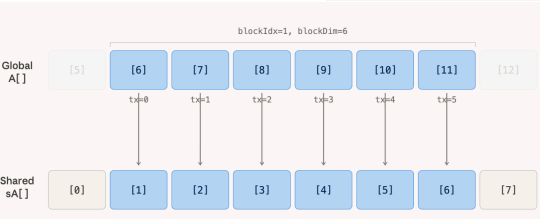
\includegraphics[width=0.7\linewidth]{images/shared.png}
    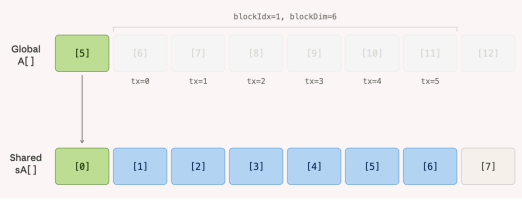
\includegraphics[width=0.7\linewidth]{images/sharedhalo.png}
    \caption{
    Mapping of global memory array \texttt{A[]} to shared memory array \texttt{sA[]} 
    in the \texttt{stencil\_shared} kernel for \texttt{blockDim.x = 6} and 
    \texttt{blockIdx.x = 1}. Threads with indices $tx \in [0,5]$ load the central 
    elements $\texttt{A}[i]$ into $\texttt{sA}[tx+1]$ for $i \in [6,11]$. 
    Additionally, halo elements are loaded such that $\texttt{sA}[0] = \texttt{A}[5]$ 
    (left halo) and $\texttt{sA}[7] = \texttt{A}[12]$ (right halo). 
    A synchronization barrier (\texttt{\_\_syncthreads()}) ensures all data is 
    available before performing the stencil computation.
    }
    \label{fig:stencil-shared-mapping}
    
\end{figure}

% ── 5.1 ──────────────────────────────────────────────────────────────────────
\subsection{Mistake 1: Using Shared Memory When There Is No Data Reuse}
\label{subsec:no-reuse}

Shared memory is a fast, on-chip resource whose primary purpose is to
\emph{eliminate redundant reads from global memory} when multiple threads
within a block access the same data element. If a particular data element
stored in shared memory is \emph{not} going to be reused across multiple
threads in the computation, there is no benefit to placing it in shared
memory.

\begin{ppkey}
  \\The justification for using shared memory is \textbf{reuse}: when many
  threads read the same element, staging it in shared memory turns $k$ slow
  global-memory reads into one global-memory read plus $k$ fast shared-memory
  reads. Shared memory also serves as an \emph{inter-thread communication
  channel} --- threads in the same block can write results into shared memory
  and have other threads read them, which is itself a form of reuse. \textbf{No
  reuse~$\Rightarrow$ no need for shared memory.}
\end{ppkey}

\begin{pppitfall}
  \\Many programmers reflexively place data in shared memory even when there is
  no reuse in their computation. This wastes a scarce, hardware-limited
  resource without any performance benefit.
\end{pppitfall}

% ── 5.2 ──────────────────────────────────────────────────────────────────────
\subsection{Mistake 2: Forgetting \texttt{\_\_syncthreads()} and Introducing
Race Conditions}
\label{subsec:forgotten-sync}

After data is written into shared memory by one thread, other threads that
subsequently read that location must be guaranteed to see the written value.
Without an explicit \texttt{\_\_syncthreads()} barrier between the write and
the read phases, the execution order of threads within a block is
non-deterministic, and a thread may read stale or uninitialised data.

\begin{pppitfall}
  \\Omitting \texttt{\_\_syncthreads()} after shared-memory writes creates a
  \textbf{race condition}: a reading thread may execute before the writing
  thread has completed its store. The bug is typically non-deterministic and
  may only manifest on certain GPU generations or under certain occupancy
  conditions.
\end{pppitfall}

The stencil example illustrates the canonical usage pattern:

\begin{ppprogram}{Correct use of \texttt{\_\_syncthreads()} in the
stencil kernel (from lecture slide 10).}{lst:label}
\begin{lstlisting}
// --- Phase 1: load halo elements into shared memory ---
if (tx == 0 && i > 0)
    sA[0] = A[i - 1];               // left halo

if (tx == blockDim.x - 1 && i < N - 1)
    sA[blockDim.x + 1] = A[i + 1];  // right halo

__syncthreads();   // <-- barrier: all shared-memory writes MUST be
                   //     visible to all threads before continuing

// --- Phase 2: compute stencil using shared memory ---
if (i > 0 && i < N - 1)
    B[i] = sA[tx] + sA[tx + 1] + sA[tx + 2];
\end{lstlisting}
\end{ppprogram}

\texttt{\_\_syncthreads()} acts as both an \textbf{execution barrier} (no
thread advances past the call until all threads in the block have reached it)
and a \textbf{memory-ordering fence} (all writes performed by all threads
before the barrier are guaranteed to be visible to all threads after the
barrier).

% ── 5.3 ──────────────────────────────────────────────────────────────────────
\subsection{Mistake 3: Allocating Too Much Shared Memory Per Block ---
Reducing SM Occupancy}
\label{subsec:sm-occupancy}

Each Streaming Multiprocessor (SM) has a fixed, hardware-limited pool of
shared memory. On modern GPUs such as the A100 or H100, an SM can schedule up
to 32 concurrent thread blocks. The shared memory consumed by \emph{each} block
is deducted from the SM's total pool. If a single block requests a large amount
of shared memory, fewer blocks can co-reside on the SM simultaneously.

\begin{ppkey}
  \\\textbf{SM occupancy} is the ratio of the number of active warps to the
  maximum number of warps an SM can support. Low occupancy means the SM has
  fewer warps available to hide memory-access latency, which directly harms
  throughput. The limiting resource can be registers, shared memory, or the
  maximum block count --- whichever is exhausted first.
\end{ppkey}

\begin{ppexample}
  \\Suppose an SM supports up to 32 concurrent
  blocks and has 48\,KB of shared memory. If each block allocates 24\,KB, then
  only $\lfloor 48\,\text{KB} / 24\,\text{KB} \rfloor = 2$ blocks can be
  scheduled concurrently, regardless of whether register pressure or other limits
  would otherwise allow more. The programmer should therefore profile and
  experiment with shared-memory allocation size to find the sweet spot between
  data reuse and occupancy.
\end{ppexample}

% ── 5.4 ──────────────────────────────────────────────────────────────────────
\subsection{Mistake 4: Bank Conflicts}
\label{subsec:bank-conflicts}

\subsubsection{How Shared Memory Is Organised in Hardware}

Shared memory is not a single monolithic array; it is physically divided into
\textbf{banks} (also referred to as \emph{streams} during the lecture). On
NVIDIA GPUs there are typically \textbf{32 banks}. Memory addresses are
interleaved across banks in a round-robin fashion: address~0 resides in
bank~0, address~1 in bank~1, \ldots, address~31 in bank~31, address~32 back
in bank~0, and so on. All banks can be accessed \emph{simultaneously} in a
single cycle, providing the high bandwidth that makes shared memory fast.

\begin{figure}[!h]
    \centering
    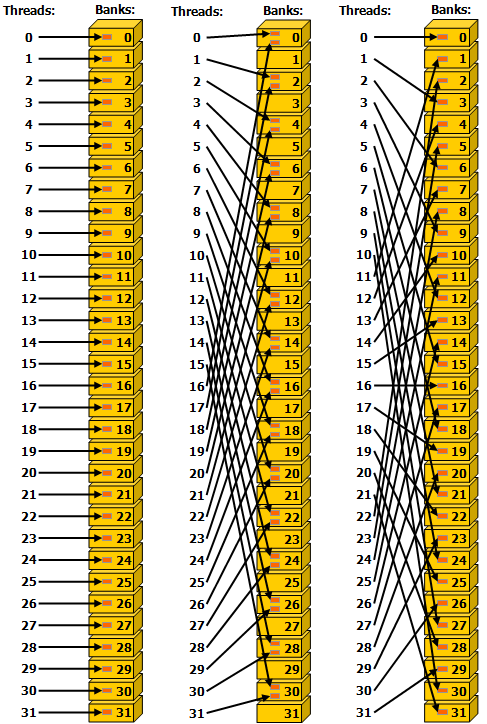
\includegraphics[width=0.75\linewidth]{images/examples-of-strided-shared-memory-accesses.png}
    \caption{
    access patterns for stride 1, 2 and 3
    }
    \label{fig:shared-memory-banks}
\end{figure}
\subsubsection{What Is a Bank Conflict?}

A \textbf{bank conflict} occurs when two or more threads within the same warp
attempt to access \emph{different addresses that map to the same bank} in the
same memory transaction. Because each bank can service only one address per
cycle, conflicting accesses must be \emph{serialised} --- the parallelism of
the warp is lost for that access. Two conflicting accesses become two serial
accesses; $n$-way conflicts result in $n$ serial accesses.

\begin{pppitfall}
  \\Even though the threads are logically concurrent, bank conflicts cause their
  memory accesses to be \textbf{serialised} at the hardware level. This
  eliminates the bandwidth advantage of shared memory and can severely degrade
  kernel performance.
\end{pppitfall}

\subsubsection{Stride and Bank Conflicts}

The access pattern that determines whether conflicts occur is characterised by
the \textbf{stride} --- the distance (in elements) between the locations
accessed by successive threads:

\begin{itemize}
  \item \textbf{Stride 1} (consecutive): thread $i$ accesses element $k$,
        thread $i+1$ accesses element $k+1$, etc. Each thread accesses a
        distinct bank. \emph{No conflicts.}
  \item \textbf{Stride $s$}: thread $i$ accesses element $k$, thread $i+1$
        accesses element $k + s$. If $s$ is a divisor of the number of banks
        (e.g.\ stride 2 with 32 banks), every other bank is skipped, and
        pairs of threads collide on the same bank. \emph{2-way conflict.}
  \item \textbf{Stride 32} (or any multiple of 32): all 32 threads in a warp
        map to the \emph{same} bank. \emph{32-way conflict --- fully
        serialised.}
\end{itemize}

The instructor noted that the exact bank-allocation policy is
\emph{proprietary} for NVIDIA hardware, but that OpenCL documentation provides
a publicly accessible description of the analogous mechanism. The general
principle --- contiguous elements map to successive banks in a round-robin
manner --- holds across vendors.

\begin{ppnote}
  \\\textbf{Student question:} How are banks actually allocated today?\\[4pt]
  \textbf{Instructor:} The detailed allocation policy is hardware-specific and
  largely proprietary for NVIDIA. In OpenCL it is documented more openly, and
  the intuitive model is round-robin: $A[0]$ in stream/bank~1, $A[1]$ in
  bank~2, $\ldots$, and once the banks are exhausted it wraps back around. So
  if your stride of access is~1, each successive thread hits a different bank
  --- no conflict. Some conflicts are \emph{inevitable} depending on the
  workload, but the programmer's obligation is to \emph{minimise} them by
  choosing the stride of access wisely. Changing the stride is within the
  programmer's control; the number of banks is fixed by the hardware engineers.
  This is a core GPU optimisation strategy.
\end{ppnote}

\subsubsection{Relationship to False Sharing in CPU Caches}

The instructor drew a direct analogy with \emph{false sharing} in CPU cache
systems. In a CPU cache, two threads updating different variables that happen
to reside on the same cache line cause that line to be repeatedly invalidated.
In shared memory the invalidation mechanism does not apply, but the outcome is
similar: concurrent accesses that fall on the same bank are \emph{serialised},
eliminating the benefit of concurrent execution.


% ─────────────────────────────────────────────────────────────────────────────
\newpage
\section{Synchronisation Primitives}
\label{sec:sync-primitives}
% ─────────────────────────────────────────────────────────────────────────────

\subsection{Overview}

CUDA provides a hierarchy of synchronisation primitives that operate at
different scopes: the warp, the thread block, the device, and the entire
system (device~+~host). Choosing the right primitive is important for both
correctness and performance --- using a coarser primitive than necessary wastes
cycles; using a finer one than required introduces data races.

The instructor categorised the primitives into two families:

\begin{enumerate}[noitemsep]
  \item \textbf{Execution barriers} --- every participating thread must arrive
        at the barrier before any may proceed.
  \item \textbf{Memory fence primitives} --- flush the calling thread's pending
        writes to the appropriate visibility scope, \emph{without} blocking
        execution of other threads.
\end{enumerate}

% ── 6.1 ──────────────────────────────────────────────────────────────────────
\subsection{\texttt{\_\_syncwarp()}: Warp-Level Synchronisation}
\label{subsec:syncwarp}

\subsubsection{Background: Warp Execution and Independent Thread Scheduling}

Historically, threads within a warp were said to execute in \emph{lock-step}:
all 32 lanes issue and retire the same instruction simultaneously. Under pure
lock-step semantics, a write by lane~$i$ followed by a read by lane~$j$ within
the same warp required no explicit synchronisation, because the write always
completes before the read begins.

Modern GPU architectures (Volta and later) introduced \textbf{Independent
Thread Scheduling} (ITS): the hardware may schedule threads within a warp with
different latencies and may interleave their execution. The lock-step guarantee
no longer holds in general, and programs that relied on it silently can now
exhibit incorrect behaviour.

\begin{ppkey}
  \\\texttt{\_\_syncwarp()} was introduced \emph{because} ITS broke the implicit
  lock-step synchronisation assumption. If the hardware truly enforced lock-step
  execution for every warp without exception, there would be no reason to
  provide the primitive. Its existence is the hardware's acknowledgement that
  the assumption can be violated.
\end{ppkey}

\begin{ppnote}
  \\\textbf{Student question:} If warps execute in lock-step, why do we need
  \texttt{\_\_syncwarp} at all?\\[4pt]
  \textbf{Instructor:} Modern GPUs perform independent thread scheduling and
  other optimisations that break the strict lock-step semantics. If the hardware
  did not have that feature at all, there would be no reason to provide
  \texttt{\_\_syncwarp}. Its presence in the API is itself the signal that the
  lock-step assumption can no longer be taken for granted.
\end{ppnote}

\subsubsection{Semantics}

\texttt{\_\_syncwarp()} acts as \emph{both} an \textbf{execution barrier}
(threads within the warp wait for each other at this point) and a
\textbf{memory fence} (prior writes become visible to all lanes in the warp).
Its cost is much lower than \texttt{\_\_syncthreads()} because it operates
only within a single warp of 32 threads.

\subsubsection{Typical Use Pattern}

Use \texttt{\_\_syncwarp()} when:
\begin{itemize}[noitemsep]
  \item The computation involves only the 32 threads of a single warp (and
        additional threads are either absent or idle).
  \item Work is split into a \emph{write phase} followed by a \emph{read
        phase} within the same warp.
  \item A full \texttt{\_\_syncthreads()} would be correct but unnecessarily
        expensive.
\end{itemize}

The following listing reproduces the example from slide~12:

\begin{ppprogram}{\texttt{\_\_syncwarp()} example: warp-level
prefix sum (from lecture slide 12).}{lst:label}
\begin{lstlisting}
int lane = threadIdx.x % 32;

// Only the first warp (threads 0..31) participates
if (threadIdx.x < 32) {
    s[lane] = A[lane];   // Phase 1: each lane loads one element

    __syncwarp();         // Barrier + fence within the warp
                          // Ensures all loads complete before reads below

    if (lane > 0)
        B[lane] = s[lane] + s[lane - 1];  // Phase 2: read neighbour's value
}
\end{lstlisting}
\end{ppprogram}

\begin{ppkey}
  \\The predicate \texttt{if (threadIdx.x < 32)} restricts the computation to
  the first warp. This is intentional: because \texttt{s[]} is in shared
  memory and $s[\text{lane} - 1]$ is written by a \emph{different} lane, the
  two phases must be separated by a synchronisation point. Within the first
  warp, \texttt{\_\_syncwarp()} is cheaper than \texttt{\_\_syncthreads()}.
\end{ppkey}

% ── 6.2 ──────────────────────────────────────────────────────────────────────
\subsection{\texttt{\_\_syncthreads()}: Block-Level Synchronisation}
\label{subsec:syncthreads}

\texttt{\_\_syncthreads()} is the most commonly used synchronisation barrier
in CUDA. It establishes a rendezvous point for \emph{all} threads in a thread
block: no thread may execute instructions beyond the barrier until every thread
in the block has arrived.

\subsubsection{Semantics (from slide 10)}

\begin{itemize}
  \item \textbf{Execution barrier:} Every thread in the block waits at the
        barrier. No thread advances until all threads have reached it.
  \item \textbf{Memory ordering:} All writes by all threads before the barrier
        are guaranteed to be visible to all threads in the block after the
        barrier. This covers both shared memory and global memory accesses.
\end{itemize}

\subsubsection{Typical Use: Phased Computation}

The canonical pattern is a computation that proceeds in two or more phases,
where phase~$k+1$ depends on results produced in phase~$k$ by \emph{all}
threads:

\begin{ppprogram}{Canonical two-phase shared-memory pattern using
\texttt{\_\_syncthreads()}.}{lst:label}
\begin{lstlisting}
// Phase 1: all threads populate shared memory
sA[tx + 1] = A[i];
if (tx == 0 && i > 0)            sA[0]            = A[i - 1];
if (tx == blockDim.x - 1 && i < N - 1) sA[blockDim.x + 1] = A[i + 1];

__syncthreads();   // <-- all phase-1 writes must be complete before
                   //     any thread reads sA[] in phase 2

// Phase 2: all threads read from shared memory
if (i > 0 && i < N - 1)
    B[i] = sA[tx] + sA[tx + 1] + sA[tx + 2];
\end{lstlisting}
\end{ppprogram}

\subsubsection{When \emph{Not} to Use \texttt{\_\_syncthreads()}}

The instructor emphasised three situations in which \texttt{\_\_syncthreads()}
must \emph{not} be used (from slide 13):

\paragraph{1. When threads are completely independent.}
If no thread in the block reads data written by another thread, no
synchronisation is necessary. Adding an unnecessary \texttt{\_\_syncthreads()}
wastes cycles waiting for all threads to arrive.

\paragraph{2. When only one warp is involved.}
Within a single warp, ITS aside, the hardware provides execution ordering at a
finer granularity. Use \texttt{\_\_syncwarp()} instead --- it is cheaper.

\paragraph{3. Inside a divergent control flow.}
\texttt{\_\_syncthreads()} \emph{must} be reached by \textbf{all} threads in
the block, unconditionally. Placing it inside a conditional branch where some
threads take the \texttt{then} path and others take the \texttt{else} path
results in \emph{deadlock or undefined behaviour}.

\begin{pppitfall}
  \\The following code is \textbf{incorrect}:
\begin{lstlisting}[numbers=none]
if (threadIdx.x < 128) {
    __syncthreads();   // WRONG: threads 128..blockDim.x-1 never reach here
}
\end{lstlisting}
  Only the first 128 threads call \texttt{\_\_syncthreads()}; the remaining
  threads do not. The barrier can never be satisfied and the kernel hangs
  (or produces undefined results, depending on the GPU generation).
\end{pppitfall}

\begin{ppnote}
  \\\textbf{Student question:} Should \texttt{\_\_syncthreads()} also be
  accompanied by \texttt{\_\_threadfence\_block()} to ensure visibility?\\[4pt]
  \textbf{Instructor:} \texttt{\_\_syncthreads()} is implemented to do both
  jobs internally --- it acts as an execution barrier \emph{and} a memory
  fence at the block scope. You do not need to call
  \texttt{\_\_threadfence\_block()} separately when you use
  \texttt{\_\_syncthreads()}.
\end{ppnote}

% ── 6.3 ──────────────────────────────────────────────────────────────────────
\subsection{Memory Fence Primitives}
\label{subsec:threadfence}

Memory fence primitives differ fundamentally from execution barriers:

\begin{center}
\renewcommand{\arraystretch}{1.3}
\begin{tabular}{@{}lll@{}}
  \toprule
  \textbf{Property} & \textbf{Execution Barrier} & \textbf{Memory Fence} \\
  \midrule
  Blocks calling thread? & Yes --- waits for others & No \\
  Blocks other threads? & Yes --- until all arrive & No \\
  Guarantees visibility? & Yes & Yes (for calling thread's \\&&writes only) \\
  Scope & All threads in group & Configurable \\
  \bottomrule
\end{tabular}
\end{center}

A memory fence causes the \emph{calling thread's} prior writes to become
visible to threads in the specified scope. It does \emph{not} wait for other
threads to reach the same point.

\begin{ppkey}
  \\Use a memory fence when you have determined, through analysis of your
  algorithm, that only \emph{some} threads need to observe a subset of writes,
  and a full barrier would stall threads unnecessarily. This gives finer-grained
  control than \texttt{\_\_syncthreads()} but demands a deeper understanding of
  the data-flow in the kernel.
\end{ppkey}

The instructor cautioned that memory fences are powerful but error-prone: used
incorrectly, they \emph{can} introduce data races by giving the programmer the
illusion of synchronisation while leaving some reads unsatisfied.

\subsubsection{\texttt{\_\_threadfence\_block()}}


\textbf{Scope:} The calling thread's prior writes become visible to all other
threads in the \emph{same block}, wherever they are in the control flow.
This is a strict subset of what \texttt{\_\_syncthreads()} provides: it does
not stall the calling thread and does not wait for other threads.

\paragraph{Example use case.}
Consider a reduction within a block where only thread~0 produces a final
result. After thread~0 writes the result to shared memory, calling
\texttt{\_\_threadfence\_block()} ensures that other threads in the block will
subsequently see the updated value, without requiring a full barrier.

\subsubsection{\texttt{\_\_threadfence()}}



\textbf{Scope:} The calling thread's prior writes become visible to \emph{all
threads on the device}, regardless of which block they belong to. This is the
device-wide memory fence.

\paragraph{Example use case.}
When a kernel uses a global flag or counter that one block writes and another
block reads (e.g.\ in a hand-written reduction across blocks), calling
\texttt{\_\_threadfence()} after writing the flag ensures that any thread on
the device that subsequently reads the flag will see the updated value.

\begin{ppnote}
  \\\textbf{Instructor (unprompted):} In most GPU programs you will not see
  \texttt{\_\_threadfence}. It is a very powerful primitive, but the power it
  gives you also means that if you use it incorrectly, you may introduce data
  races. What the fence does is reflect all writes that have happened in the
  past by the calling thread into the appropriate memory scope --- it does not
  by itself prevent another thread from concurrently writing to the same
  location. You still have to reason carefully about your algorithm.
\end{ppnote}

\subsubsection{\texttt{\_\_threadfence\_system()}}


\textbf{Scope:} The calling thread's prior writes become visible not only to
all threads on the device but also to \emph{threads on the host (CPU)}.
Internally, this requires a \textbf{device-to-host data transfer} to flush
the GPU write buffers through the PCIe bus and into host-visible memory.

\begin{pppitfall}
  \\\texttt{\_\_threadfence\_system()} is the most expensive memory primitive in
  the CUDA hierarchy. Because it triggers a device-to-host transfer for every
  calling thread that executes it, it should be used only when a GPU thread
  genuinely needs to signal the CPU, not as a general-purpose fence.
\end{pppitfall}



% ── 6.4 ──────────────────────────────────────────────────────────────────────
\subsection{Choosing the Right Primitive: Decision Heuristics}
\label{subsec:choosing}

The following heuristics, drawn from the lecture discussion, guide the
selection of the appropriate primitive:

\begin{enumerate}
  \item \textbf{Are the threads completely independent?} Use no primitive.
        Adding any synchronisation where it is not needed only wastes cycles.

  \item \textbf{Is the computation confined to one warp?} Use
        \texttt{\_\_syncwarp()} instead of \texttt{\_\_syncthreads()}. The
        latter is a ``heavy hammer'' when only 32 threads are involved.

  \item \textbf{Do all threads in the block participate, in phases?} Use
        \texttt{\_\_syncthreads()}.

  \item \textbf{Only some threads write; others need to observe those
        writes --- but no full rendezvous is needed?} Consider
        \texttt{\_\_threadfence\_block()}. Ensure that the reading threads
        will actually execute \emph{after} the fence (e.g.\ because they are
        in a different kernel phase or the write happens at a known point in
        the control flow).

  \item \textbf{Writes need to be visible across blocks on the same device?}
        Use \texttt{\_\_threadfence()}.

  \item \textbf{A GPU thread must signal the CPU?} Use\\
        \texttt{\_\_threadfence\_system()}, but be aware of the transfer cost.
\end{enumerate}

\begin{ppnote}
  \\\textbf{Student question:} Does using a memory fence introduce data races?\\[4pt]
  \textbf{Instructor:} The fence itself does not introduce a data race --- it
  makes the calling thread's past writes visible. However, the fence gives
  you enough rope to hang yourself: it only flushes \emph{one} thread's
  writes. If you assume that the fence simultaneously prevents another thread
  from writing to the same location, you will have a race. Understanding
  exactly what your workload requires is the programmer's responsibility.
  ChatGPT and Claude will not do that reasoning for you.
\end{ppnote}

% ── 6.5 ──────────────────────────────────────────────────────────────────────
\subsection{Practice Assignment: Producer--Consumer with Thread Fences}
\label{subsec:assignment}

The instructor concluded the synchronisation-primitives discussion with the
following \textbf{ungraded practice assignment}:

\begin{tcolorbox}[colback=blue!5,
  title=\textbf{Practice Assignment (Ungraded)},fonttitle=\small\bfseries]
  Write a simple \emph{producer--consumer} kernel using the different memory
  fence primitives:
  \begin{enumerate}[noitemsep]
    \item Implement the pattern using \texttt{\_\_threadfence\_block()}.
    \item Implement it using \texttt{\_\_threadfence()}.
    \item Implement it using \texttt{\_\_threadfence\_system()}.
  \end{enumerate}
  Ensure each version is \emph{correct} (no data races). Then measure and
  compare the execution times of the three versions. Articulate, in writing,
  why one fence is more efficient than the others for this workload and what
  the trade-off is between the scope of visibility and the overhead of the
  fence operation.
\end{tcolorbox}

\subsection{Exercises}
\begin{ppexercises}

\ppexercise{%
  \textbf{Common Mistakes --- Identification:} For each of the four kernel snippets below, identify \emph{which} common shared-memory mistake (if any) is present and briefly explain the consequence.

  \begin{enumerate}[label=(\alph*)]
    \item A kernel copies each element of a global array into shared memory, reads it back once, and writes the result directly to a second global array. No element is read by more than one thread.
    \item A kernel loads a tile of a matrix into shared memory and then immediately (without any barrier) uses those shared-memory values to compute a dot product.
    \item Each block allocates \ppinline{\_\_shared\_\_ float buf[32768];} (128\,KB) on an SM that has only 48\,KB of shared memory per SM.
    \item Threads in a warp access \ppinline{sA[threadIdx.x * 32]} (stride-32 access into a 32-bank shared-memory array).
  \end{enumerate}
}

\ppexercise{%
  \textbf{Synchronisation Primitive Selection:} For each scenario, choose the \emph{most appropriate} CUDA synchronisation primitive from the list
  \{\ppinline{\_\_syncwarp()}, \ppinline{\_\_syncthreads()}, \ppinline{\_\_threadfence\_block()}, \ppinline{\_\_threadfence()}, \ppinline{\_\_threadfence\_system()}\}
  and justify your choice.

  \begin{enumerate}[label=(\alph*)]
    \item All 256 threads of a block cooperatively fill a shared-memory tile in Phase~1 and then read from it in Phase~2.
    \item Only the 32 threads of the first warp participate in a warp-level prefix sum using shared memory.
    \item Thread~0 of a block writes a ``done'' flag into shared memory. Other threads in the \emph{same block} will poll that flag later in the kernel, but no barrier rendezvous is needed or desired.
    \item Block~0 computes a partial result and writes it to a global variable. Block~1 must read that global variable \emph{after} Block~0 has written it (within a single kernel launch, assuming cooperative groups are not used).
    \item A GPU thread writes a result to pinned (page-locked) host memory that the CPU will read immediately after a host-side polling loop.
  \end{enumerate}
}

\ppexercise{%
  \textbf{Divergent \texttt{\_\_syncthreads()} and Fix:} Consider the following kernel intended to perform two different shared-memory operations depending on thread index (Code is given below):



  \begin{enumerate}[label=(\alph*)]
    \item Explain precisely why this kernel is incorrect. Which of the four common shared-memory mistakes does it illustrate?
    \item Will the kernel always hang, or only sometimes? Explain.
    \item Rewrite the kernel so that it is correct: both halves of the computation are performed, no thread is left waiting at an unsatisfiable barrier, and the intended shared-memory reads are safe.
  \end{enumerate}
}

\end{ppexercises}
\begin{lstlisting}[language=C++]
__global__ void broken_kernel(float *A, float *B, float *C, int N) {
    __shared__ float s[256];
    int tx = threadIdx.x;
    int i  = blockIdx.x * blockDim.x + tx;

    if (tx < 128) {
        s[tx] = A[i];
        __syncthreads();          // (X)
        C[i] = s[tx] + s[tx + 1];
    } else {
        s[tx] = B[i];
        __syncthreads();          // (Y)
        C[i] = s[tx] + s[tx - 1];
    }
}
\end{lstlisting}
\section*{Solutions}

\subsubsection{Solution 1}

\begin{enumerate}[label=(\alph*)]
  \item \textbf{Mistake~1 --- No data reuse.}  Each shared-memory slot is written
        by exactly one thread and read by exactly one thread (the same thread).
        There is zero reuse across threads, so staging the data in shared memory
        provides no performance benefit and wastes on-chip capacity.

  \item \textbf{Mistake~2 --- Missing \ppinline{\_\_syncthreads()}.}  The tile
        load and the dot-product computation are in the same phase with no barrier
        between them.  A thread may begin reading shared-memory values written by
        \emph{other} threads before those writes have completed, producing a race
        condition and incorrect results.

  \item \textbf{Mistake~3 --- Excessive shared memory per block.}  128\,KB exceeds
        the SM's 48\,KB pool entirely; the kernel will fail to launch
        (\ppinline{cudaErrorInvalidValue} or similar).  Even if the request were
        smaller but still large relative to the pool, it would drastically reduce
        the number of blocks that can co-reside on the SM, lowering occupancy and
        throughput.

  \item \textbf{Mistake~4 --- Bank conflict.}  With 32 banks and a stride of 32,
        every thread in the warp maps to \emph{bank 0} (since
        $(\texttt{threadIdx.x} \times 32) \bmod 32 = 0$ for all threads).  This
        is a 32-way conflict: the 32 accesses are fully serialised, eliminating
        all shared-memory bandwidth benefit.
\end{enumerate}

\subsubsection{Solution 2}

\begin{enumerate}[label=(\alph*)]
  \item \ppinline{\_\_syncthreads()}.  All 256 threads participate, the computation
        is phased (fill then read), and every thread must have completed its write
        before any thread begins reading.  A block-wide barrier + fence is required.

  \item \ppinline{\_\_syncwarp()}.  Only 32 threads (one warp) are involved.
        \ppinline{\_\_syncthreads()} would also be correct but wastes cycles
        synchronising the other warps in the block that are not participating.
        \ppinline{\_\_syncwarp()} provides the same barrier + fence guarantee at
        warp scope for a fraction of the cost.

  \item \ppinline{\_\_threadfence\_block()}.  A full barrier is not desired
        (other threads should not stall).  Only thread~0's write needs to become
        visible to the rest of the block.  \ppinline{\_\_threadfence\_block()}
        flushes thread~0's write to block-scope visibility without blocking
        execution of any thread.

  \item \ppinline{\_\_threadfence()}.  The write must be visible across thread
        \emph{blocks} on the same device.  \ppinline{\_\_syncthreads()} only
        synchronises within one block and cannot coordinate between blocks.
        \ppinline{\_\_threadfence()} makes the calling thread's writes visible
        device-wide.  (Note: even with the fence, the programmer must ensure
        that Block~1 reads the variable \emph{after} Block~0 has written and
        fenced it --- ordering between blocks requires additional signalling
        logic such as an atomic flag.)

  \item \ppinline{\_\_threadfence\_system()}.  The write must cross the PCIe bus
        and become visible to the \emph{host CPU}.
        \ppinline{\_\_threadfence()} only guarantees device-scope visibility;
        \ppinline{\_\_threadfence\_system()} is the only primitive that flushes
        GPU write buffers all the way into host-visible memory.  It is expensive
        and should be used sparingly.
\end{enumerate}

\subsubsection{Solution 3}

\begin{enumerate}[label=(\alph*)]
  \item The kernel places \ppinline{\_\_syncthreads()} inside a divergent
        \ppinline{if}-\ppinline{else} branch.  Threads~0--127 reach barrier~(X)
        inside the \ppinline{then} branch; threads~128--255 reach barrier~(Y)
        inside the \ppinline{else} branch.  \ppinline{\_\_syncthreads()} requires
        \emph{all} threads in the block to arrive at the \emph{same} barrier
        instance.  Because the two groups arrive at \emph{different} barrier
        instances, the condition can never be satisfied.  This is
        \textbf{Mistake~2} (missing/misused \ppinline{\_\_syncthreads()}) combined
        with the specific sub-case of divergent control flow.

  \item On most GPU generations the kernel will \textbf{hang} (deadlock)
        deterministically, not just sometimes.  The CUDA specification states that
        placing \ppinline{\_\_syncthreads()} in divergent code results in undefined
        behaviour; in practice, the SM stalls waiting for a barrier that is never
        collectively reached.

  \item The fix is to move both stores \emph{before} a single, unconditional
        barrier and then move the divergent reads \emph{after} it:

\begin{lstlisting}[language=C++]
__global__ void fixed_kernel(float *A, float *B, float *C, int N) {
    __shared__ float s[256];
    int tx = threadIdx.x;
    int i  = blockIdx.x * blockDim.x + tx;

    // Phase 1: all threads write to shared memory (no divergence)
    if (tx < 128)
        s[tx] = A[i];
    else
        s[tx] = B[i];

    // Single unconditional barrier: all 256 writes must complete
    __syncthreads();

    // Phase 2: divergent reads are now safe
    if (tx < 128)
        C[i] = s[tx] + s[tx + 1];
    else
        C[i] = s[tx] + s[tx - 1];
}
\end{lstlisting}

        The single \ppinline{\_\_syncthreads()} is now reached unconditionally by
        all threads; Phase~1 stores by both halves of the block are guaranteed
        visible before any Phase~2 read executes.
\end{enumerate}

% ─────────────────────────────────────────────────────────────────────────────
\newpage
\section{End-of-Lecture Notes}

% ─────────────────────────────────────────────────────────────────────────────

The instructor also announced that TAs would release a \textbf{practice
problem set of 10 questions} on shared memory, \texttt{\_\_syncthreads()},
and device synchronisation. Problems include tasks such as implementing a
matrix transpose using shared memory. Students are encouraged to complete this
set to consolidate the concepts from Lectures 15 and 16.

\vspace{8pt}

\begin{tcolorbox}[colback=gray!8,colframe=gray!50,
  title=\textbf{Quick-Reference: Synchronisation Primitives (Slide 14)},
  fonttitle=\small\bfseries]
\begin{itemize}[noitemsep]
  \item \textbf{\texttt{\_\_syncwarp()}} --- Warp-level barrier + fence.
        Avoids the cost of a full block barrier when only one warp is involved.
  \item \textbf{\texttt{\_\_syncthreads()}} --- Block-level barrier + fence.
        All block threads must finish one phase before any may begin the next.
        \emph{Do not use} inside divergent control flow, when threads are
        independent, or when only one warp is active.
  \item \textbf{\texttt{\_\_threadfence\_block()}} --- Memory fence: calling
        thread's prior writes become visible to all threads of the block.
  \item \textbf{\texttt{\_\_threadfence()}} --- Memory fence: calling thread's
        prior writes become visible to all threads of the device.
  \item \textbf{\texttt{\_\_threadfence\_system()}} --- Memory fence: calling
        thread's prior writes become visible to all threads of the device
        \emph{and} to the host. Most expensive; requires a device-to-host
        transfer.
\end{itemize}
\end{tcolorbox}
\newpage
\section {References}
\begin{itemize}
    \item COL 380 - Subodh Sharma, \textit{Introduction to Parallel and Distributed Programming}, Course slides.
    \item Ruud van der Pas, \textit{Tasking in OpenMP}, SC13 Tutorial Slides, OpenMP Architecture Review Board. \url{https://www.openmp.org/wp-content/uploads/sc13.tasking.ruud.pdf}
    \item Ananth Grama, Georg Karypis, Vipin Kumar, and Anshul Gupta, \textit{Introduction to Parallel Computing}, Addison-Wesley.
    \item Subodh Kumar, \textit{Introduction to Parallel Programming}, Lecture Notes.
    \item Peter S. Pacheco, \textit{An Introduction to Parallel Programming}, Morgan Kaufmann.
\end{itemize}

\section{Contribution Statement}

\begin{itemize}
    \item \textbf{Rajat Soni (2023CS10229)} \begin{itemize}
        \item Documented the Shared memory usage part (Slides 8--10).
        \item Wrote Excercise and Solutions for the shared memory usage part.
        \item Developed a comprehensive verbatim transcript of the lecture.
        \item Compiled and formatted all bibliographic references.
    \end{itemize}
    \item \textbf{Chunduru Yagneshwara Naga Venkata Hanumath (2022CS11608)}
    \begin{itemize}
        \item Written the Introduction to CUDA and GPU (Slides 1--7)
        \item Documented the basics in CUDA
        \item Given examples for getting hands on cuda basics.
    \end{itemize}
     \item \textbf{Ujjawal Sharma (2022CS51137)}   \begin{itemize}
        \item Documented the Common Mistakes with Shared Memory. (Section 3.5) (Slide 11).
        \item Wrote and Explained Synchronisation Primitives with examples (Section 3.6) (Slides 12--14).
        \item Mentioned relevant class discussions and Wrote Exercises and Solutions for deep understanding.
    \end{itemize}
     \item \textbf{A. Sai Srinivas (2022CS11620)}   \begin{itemize}
        \item Wrote the Section Revisiting the Memory Hierarchy (Slide 7).
    \end{itemize}
    
\end{itemize}